\documentclass[a4paper,11pt,fleqn,twoside,notitlepage]{report}
\usepackage[utf8]{inputenc}
\usepackage{tikz}
\usepackage{float}
\usepackage[margin=2.5cm]{geometry}
\usepackage{graphicx}
\usepackage[T1]{fontenc}
\usepackage{amsmath}

\usepackage{csquotes}
\usepackage[english]{babel}
\usepackage{float}
\usepackage{caption}
\usepackage{makecell}
\usepackage{hyperref}
\usepackage{bm}
\usepackage{newfloat}
\usepackage{amsfonts}

\usetikzlibrary{calc,trees,positioning,arrows,chains,shapes.geometric,%
    decorations.pathreplacing,decorations.pathmorphing,shapes,%
    matrix,shapes.symbols}

\begin{document}

	\begin{figure}
		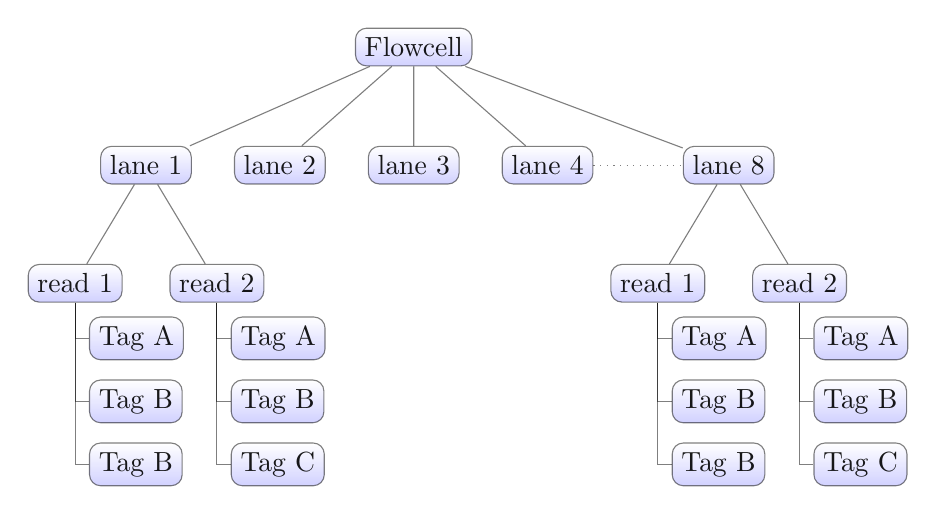
\begin{tikzpicture}[%
	sibling distance=10em,
  	every node/.style = {shape=rectangle, rounded corners,draw,align=center,top color=white, bottom color=blue!20},
    	grandchild/.style={grow=down,xshift=0.5em,anchor=west,
  	  edge from parent path={(\tikzparentnode.south) |- (\tikzchildnode.west)}},
  	grandchildRight/.style={grow=down,xshift=0.5em,anchor=west,
  	  edge from parent path={(\tikzparentnode.south) |-(\tikzchildnode.west)}},
	level 1/.style={sibling distance=17mm},
	level 2/.style={sibling distance=18mm},
	fill opacity=.9,draw opacity=.5
	]
  \node  at (-10,10) {Flowcell}
    child { node [level 1] (c1) {lane 1} 
    		child [level 2] {node {read 1}
    			child [grandchild, level distance=23mm] { node {Tag B}}	
    			child [grandchild, level distance=15mm] { node {Tag B}}
    			child [grandchild, level distance=7mm] { node {Tag A}}}
    		child [level 2] {node {read 2}
    			child [grandchildRight, level distance=23mm] { node {Tag C}}
    			child [grandchildRight, level distance=15mm] { node {Tag B}}
			child [grandchildRight, level distance=7mm] { node {Tag A}}    		
    		}}
    child [level 1] { node {lane 2} }
	child [level 1] { node {lane 3} }
	child [level 1] { node (c4) {lane 4} }
    child [sibling distance=20mm] { node (c8) {lane 8}
		child [level 2] { node {read 1}
			child [grandchild, level distance=23mm] { node {Tag B}}	
    			child [grandchild, level distance=15mm] { node {Tag B}}
    			child [grandchild, level distance=7mm] { node {Tag A}}}
    		child [level 2] {node {read 2}
    			child [grandchildRight, level distance=23mm] { node {Tag C}}
    			child [grandchildRight, level distance=15mm] { node {Tag B}}
			child [grandchildRight, level distance=7mm] { node {Tag A}}}
    		};
 \draw [dotted] (c4) -- (c8);
		\end{tikzpicture}
	\end{figure}


\end{document}